\section{Methodology}
\setlength{\parindent}{10ex}
The following chapter describes the data used in this project and how it was used for training.
Bathymetry data was extracted from the \ac{ETOPO}2v2 and used as truth value to train against a set of ocean features.
These ocean features were selected from a large set of aggregated features.
The selection was driven by a genetic algorithm that was used for speed as opposed to accuracy.
The trained models are then used to make predictions for the spatial resolution that was used in training.

\subsection{Bathymetry Data}
Data derived from predicted \ac{EGM} datasets represent the actual value of bathymetry at that point.
For example, predicted bathymetry datasets have geospatial coverage.
These coverages vary in size by the resolution of the imagery.
Higher resolution imagery will have smaller coverages, and lower resolution will have more extensive coverages.
The predicted values used in this project represent an average of bathymetry across coverage. 
These predicted datasets are used as the truth values for training, but it is important to note that they are, themselves, predicted values.
Using this data is not intended to build accurate predictors, but to show that an accurate predictor can be built.

\par
The \ac{ETOPO} dataset is used in this project for bathymetry data.
This dataset is an aggregation of sparse \ac{MBES} ship soundings and predicted bathymetry from an \ac{EGM}.
It is an updated version of the original ETOPO2 dataset and was chosen because of the two-minute resolution it offers.
\ac{ETOPO} was aggregated by the \ac{NGDC}, which is a department of \ac{NOAA}.

\par
Land topography is included in the \ac{ETOPO} dataset.
This proved to be problematic in creating accurate bathymetry predictions.
Therefore, a mask was created to remove the land topography in all training datasets.
This is applied to the data before training to ensure that land data is not used in training.

%There is a better was to describe why the features were binned like this
%I want to describe the value that was added by binning my data into classes!
\par
Classification requires discrete class labels to predict.
To accommodate this requirement, the \ac{ETOPO} dataset was binned into discrete classes.
This binning was performed at 150-meter intervals.
This partitioning scheme was chosen to compare to the results from a similar work~\cite{jena2012prediction}.

\subsection{Training Data}
All feature data was aggregated from ocean and earth studies.
This data was then normalized and formatted for this project.
This aggregation was performed to gather a large set of testing samples regardless of the data's relevance.
For example, crust age may not be obviously useful for predicting bathymetry, but if it is useful, then feature selection will identify it as such.
This approach is fundamentally different from building a physics model.
For example, the mass of a geoid causes a vertical gravity gradient, which creates ocean swells that can be measured by satellite altimetry.
Larger geoids will naturally affect the bathymetry of the sea floor.
This relationship is obvious and correlated in a measurable way.
On the other hand, machine learning can potentially identify relations in the data that otherwise will be difficult for a human to identify and model.

All features and their origin datasets can be seen in Table 1. %Insert point to figure yadaydada
Absent data points were either interpolated or filled with default values.

\par
Figure~\ref{fig:bathyxfish} shows a plot of estimated fish biomass and bathymetry.
It can be conjectured that this relationship is more correlation than causality.
For example, biomass increases are not caused by shallow depths.
The shallow depth has more available light, which allows for vegetation and energy supplies for more species, which could explain the relationship shown in this figure.

\par
Figure~\ref{fig:bathyxdensity} shows a graph of crust density and bathymetry.
This relationship may be more of causality than correlation.
The denser crust is caused by many different factors that are separate from bathymetry.
It is possible that deeper water columns and the resulting weight contributed, but it can not be used to describe the correlation of the variables.

\par
In general, the features used in this project were a collection of potential predictors.
Features such as estimated oxygen, nitrogen, and salinity make sense for being related to bathymetry.
Other features, such as crust density may not naturally be explained.
The feature selection was used to identify the best performing features.
Future studies in the relationship between these features and how they benefit predicting bathymetry will be necessary.

\begin{figure}[htp]
    \centering
    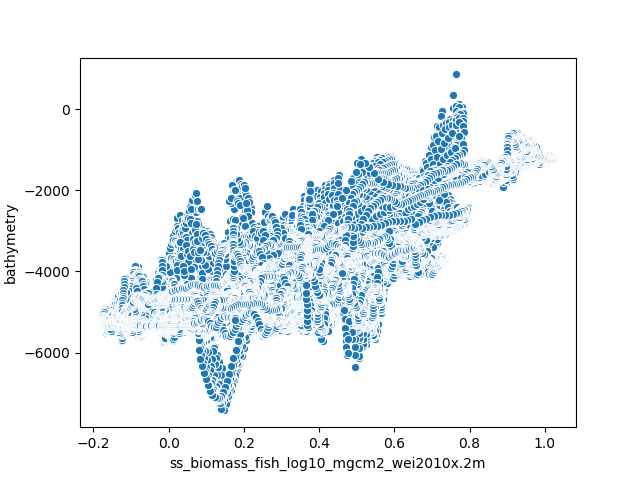
\includegraphics[width=\textwidth]{Bathymetry_X_SS_BIOMASS_FISH_LOG10_MGCM2_Wei2010x.png}
    \caption{Graph of Bathymetry and Estimated Fish BIOMASS. Bathymetry is measured in meters and Fish Biomass is measured }
    \label{fig:bathyxfish}
\end{figure}

\begin{figure}[htp]
    \centering
    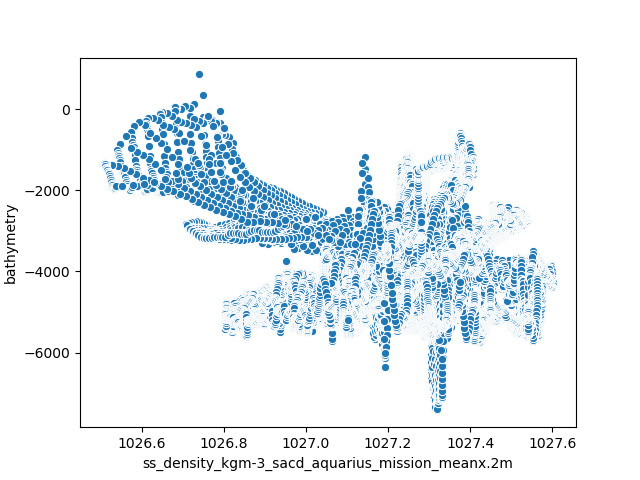
\includegraphics[width=\textwidth]{Bathymetry_X_SS_DENSITY_KGM-3_SACD_Aquarius_MISSION_MEANx.png}
    \caption{Graph of Bathymetry and Estimated Crust Density.
    Bathymetry is measured in meters, and Crust Density is measured in milligrams per squared centimeter.}
    \label{fig:bathyxdensity}
\end{figure}

%This section is for defining the data being used in the experiment
%It should define where the data came from and its format
%I can also explain any of the special stuff I am doing (Binning for example)
%

\newpage

\begin{table}[htp]
    \centering
    \caption{List of Ocean Features used in Models for this project.}
    \begin{tabular}{ |p{0.5\textwidth} p{0.5\textwidth}| }
        \hline
            \textbf{Feature} & \textbf{Origin Study} \\
            \hline
            Mantle Density & CRUST1~\cite{laske2013update} \\
            LAND One Hot & ETOPO~\cite{national1988etopo} \\
            Crust Thickness & CRUST1~\cite{laske2013update} \\
            Low, Mid, High Crust Density & CRUST1~\cite{laske2013update} \\
            Estimated Current East, North, Mag & HYCOM~\cite{chassignet2009us} \\
            Sea Nitrate, Phosphate, Salinity Measurements & NASA Studies~\cite{meissner2018salinity,parekh2005decoupling}  \\
            Sea Temperature, Silicate Measurements & NASA Studies \\
            Sediment Thickness & CRUST1~\cite{laske2013update} \\
            BioMass Features &~\cite{wei2010global} \\
            Geoid Features & EGM~\cite{pavlis2008earth} \\
            Wave height, period & WAVEWATCH~\cite{tolman20072007} \\
        \hline
    \end{tabular}
    \label{table:FEATURE_LIST}
\end{table}
%I am using this section to introduce the feature selection method that I preformed
%Maybe I can flesh this out more and talk about it in def??
%Maybe make a diagram for the flow of the GA?
\subsection{Feature Selection}
Feature selection was used to identify the most relevant features for classification.
This important step in the \ac{ML} pipeline removes noise from irrelevant data.
This work used a genetic algorithm approach for feature selection~\cite{yang1998feature}.
Other approaches that were considered included a grid search, dimensional analysis, and simple variable correlations.
These approaches were found to either take too long or simply not offer enough improvement to the model.
The genetic algorithm approach gave relatively quick model improvements with little effort.
See Figure \ref{fig:genetic} for an illustration of a generic genetic algorithm.

\par
Using a genetic algorithm for feature selection is a simple application of the original process.
The initialized population is a set of random binary strings.
Each string has a character length equal to the number of features in our feature space.
The binary characters represent whether a feature is active or inactive.
Essentially these strings represent a set of features to use in training a model.
The fitness of that string is represented by the resulting model's accuracy.
Selection is performed by choosing the most accurate models and their characteristics then passing those onto the next generation.
A simple crossover mutation of the strings is used along with a modest 5\% mutation rate.
Upon termination, the resulting fittest string is used as the selected features.


\begin{figure}[htp]
    \centering
    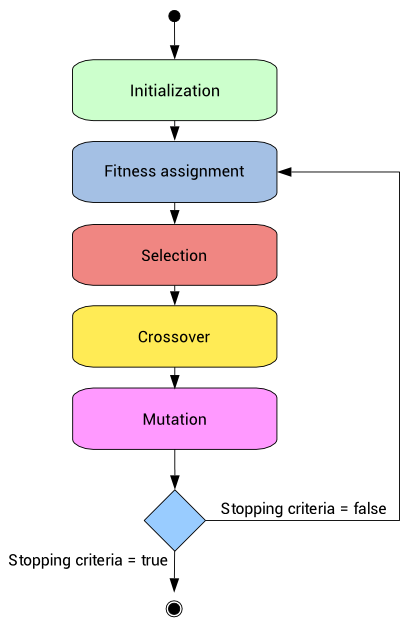
\includegraphics[scale=0.5]{genetic_algorithm.png}
    \caption{State Diagram of Generic Genetic Algorithm.
    The algorithm begins at an initialization state where the population is created.
    It then assigns a fitness attribute to each member of the population.
    This is the Fitness Assignment State.
    Then in the Selection State, a selection is performed where the highest-ranking members are selected for crossover and mutation.
    These states are designed to replenish the population.
    These actions are performed in the Crossover and Mutation States, respectively.
    Finally, a stopping criterion is evaluated.
    If the population meets this criterion, the algorithm exits; else, it goes to the Fitness Assignment State and repeats the previous steps.}
    \label{fig:genetic}
\end{figure}

\par
Feature selection was used to remove noise from the training data.
This down sizing happened on a global scale.
It is possible that this may affect localized predictions where a feature is a strong predictor.
This was not tested in this work, but it is an interesting question.
Identifying locally optimum features could lead to better models.


%This decribes how the grid files are used and oragnized...
%They are essentially binary files...
\subsection{Data Representation}
Representing the topography of the earth can be done using a grid. 
Naturally, mapping a large circular sphere to a flat grid is not a direct conversion.
Latitude and Longitude represent the grid lines for the earth.
The data in the grid is a representation of the average value across an area.
This grid representation allows for ease of reading both by computers and humans.

\par
The spatial resolution of a grid defines its coverage.
It can be described as the height and width of a grid.
This height and width are not spatially constant.
For example, a cell at the equator is larger and covers more physical area than a cell at the poles.
This format is preferred because it represents the data in a consistent and structured manner.

\par
All data in this project has been organized into two-minute bathymetry grids.
A two-minute bathymetry grid has a spatial resolution of 0.034 degrees per cell, which is approximately 3 kilometers of spatial coverage.
The grids have a column length of 5400 and a row width of 10800.
This resolution was chosen for experiments to conserve memory and time.
Larger grids have an exponentially larger memory and computational footprint.
I used the \ac{ETOPO}2v2~\cite{national1988etopo} dataset as the source of the two-minute bathymetry grid.
Finer resolution datasets exist, such as the SRMT30~\cite{becker2009global} at 30 second resolution, however, the two-minute resolution offered a good balance of memory, accuracy, and computational costs.

\subsection{Metrics}
Metrics are useful for evaluating a model and determining its usefulness.
The metrics used in this paper were chosen with this goal in mind.
RMSE, R2, F1-score, and Balanced Accuracy are the metrics used in this paper.

\par
RMSE stands for Root Mean Square Error.
It is the square of average squared error, and is ideal for aggregating the magnitudes of error.
It is given by the following equation.
\begin{equation}
    RMSE = \sqrt{\frac{1}{n}\Sigma_{i=1}^{n}{\Big(\frac{d_i -f_i}{\sigma_i}\Big)^2}}
\end{equation}

\par
R2 stands for "R Squared".
In statistics, this is the coefficient of determination, it is defined as the proportion of the variance in the dependent variable that is predictable from the independent variables.
Having a high R squared score will denote that the features of a model are good predictors.
It is given by the following equation.
\begin{equation}
    r = \frac{n(\Sigma x y)-(\Sigma x)(\Sigma y)}{\sqrt{[n \Sigma x^2  - (\Sigma x)^2][n(\Sigma y^2) - (\Sigma y)^2]}}
\end{equation}

\par
F1-Score represents a harmonic mean of a model's precision and recall.
Precision is the measurement of how good a model is at avoiding false positives.
It is known as the true positive rate.
The recall is a measurement of how good a model is at avoiding false negatives.
The equations are given below.
\begin{equation}
    precision = \frac{True Positives}{True Positives + False Positives}
\end{equation}
\begin{equation}
    recall = \frac{True Positives}{True Positives + False Negatives}
\end{equation}
\begin{equation}
    F1 = 2 * \frac{precision * recall}{precision + recall}
\end{equation}

\par
Balanced Accuracy gives an indication of accuracy for datasets that are not balanced.
A dataset that is not balanced means that one label has significantly more or fewer samples than another.
The equation is given below.
\begin{equation}
    Balanced\! Accuracy = \frac{True Positive Rate + True Negative Rate}{2}
\end{equation}





\subsection{Learning Methodology}
Supervised regression, classification models, and a novel ensemble were trained for this research.
The training was performed using previously predicted bathymetry as the truth data.
Potential predictors in the form of Ocean data were aggregated and used as training features.
Predictors that performed well were selected by a genetic algorithm.

\subsection{Regression Methodology}
Regression \ac{ML} models were fit in order to compare to existing physics models.
Three models were fit to the data: 
an SVM regression model, a Naive Bayes regression model, and a simple linear regression model.
These models were trained against a reduced set of data shown in Figure~\ref{fig:trainset}, and validated against the world-wide data not used in the training phase.
Each model was fit against selected features from the Genetic Algorithm feature selector.

\subsection{Classification Methodology}
To facilitate classification, trained models are needed to predict discrete values instead of continuous values.
This conversion was executed by mapping the bathymetry values into discrete classes.
The conversion proved to be trivial because of the ordered nature of bathymetry.
Classification models are simpler and easier to fit than regression models.
Ideally, the decision surfaces will benefit from the conversion and yield better results.
This makes it difficult to compare directly to the error reported in existing physics models.
A set of metrics, including precision, recall, F1-score, and Balanced Accuracy were used to analyze the viability of the models.

\par
The ordinal classes were binned on an interval of 150 meters.
Essentially, this gives a true positive error of approximately 150 meters.
This was done to easily compare accuracy to the model in~\cite{jena2012prediction}.
Validation was performed with 10-fold cross-validation using Balanced Accuracy as the scoring function.
The following models were imported from the Sklearn library and trained: Random Forest Classifier, Quadratic Discriminant Classifier, AdaBoost Classifier, Gradient Boosting Classifier, Decision Tree Classifier, Artificial Neural Network Classifier, Voting Classifier, KNN Classifier, Bagging Classifier, NaiveBayes Classifier.


\subsection{Model Selection Methodology}
\setlength{\parindent}{10ex}
%Purpose of this section is to identify the optimized grid structure.
%I need to check with Hoque to identify what I should and shouldnt include
%I need to consider rewording this and restructuring to manage the correctness for example etc.
% Further analysis of figure \ref{fig:rfc_report} shows that models are sensitive to potentially local characteristics.
% In an attempt to test this notion and increase the accuracy of these models a novel model selection method was employed.
% The objective being to identify if a model will predict more accuractly based on geospatial location.
% The hypothysis being that decision boundaries across different models will respond to features based on location
For optimization a grid optimization methodology was developed.
Essentially, grid optimization uses a decision function to select the best predictor.
A cache of models was used for this decision function, specifically, the cache is a map of a model to a geospatial area.
The methodology is that specific models will be better at predicting specific geospatial areas.
This cache was implemented by comparing the performance of a set of models for predicting across the globe.
For sake of time and computing resources, the world was split into \textbf{N} coverages.
These coverages represent an area of the earth and sufficed for the experiment.
Each model was trained using data contained by a radius surrounding the coverage.
Using 10-fold cross validation each model was scored and then compared.
The best performing model was then placed into the cache.
For predicting globally, each model was trained and validated against the entire dataset.

Model selection using this grid optimization methodology allowed the best predictor to be used at all times.
Figure \ref{fig:coveragegrid} shows that model accuracy varied greatly by region.
Showing evidence that there does not exist a best fit model for predicting bathymetry across the earth.
For example, consider a model that is excellent at predicting shallow bathymetry.
This model's performance could be explained by how it interprets data and models it.
Specifically, it may leverage the predictors in the data well.
However, this same model that works well in shallow water may be awful in deep water.
Whereas, another model may be excellent at predicting bathymetry in deep water scenarios.
This methodology solved this problem by always using the best predictor for an area.